\documentclass[a4paper,14pt]{extreport}

\usepackage[T1,T2A]{fontenc}
\usepackage[utf8]{inputenc}

\usepackage{title}
\usepackage{bsumain}
\usepackage{blindtext}

\usepackage{hyperref}
\usepackage{subfigure}
\usepackage[final]{graphicx}

\title{Улучшение качества видеопотока с помощью нейронных сетей на графических процессорах}
\author{Бинцаровского Леонида Петровича}
\mentor{старший преподаватель\\
        Д. И. Пирштук}

\renewcommand\contentsname{Оглавление}

\begin{document}
    \maketitle\newpage
    
    \chapter*{Реферат}
    Курсовая работа, 32 стр., 9 иллюстр., 6 источников.\\
    \textbf{Ключевые слова:} MediaPipe; C++; Swift; Metal; XNNPack; инференс.\\
    \textbf{Объекты исследования} — улучшение качества видеопотока с помощью нейронных сетей на графических процессорах.\\
    \textbf{Цель исследования} — реализация конвейера для улучшения качества видеопотока с помощью нейронных сетей на графических процессорах и приложений для тестирования данного конвейера на macOS, Linux и iOS.\\
    \textbf{Методы исследования} — системный подход, изучение соответствующей литературы и электронных источников, постановка задачи и её решение.\\
    \textbf{В результате исследования} были разработаны конвейеры для улучшения качества видеопотока на macOS, Linux и iOS. Реализованы приложения на C++ и Swift для запуска и тестирования данных конвейеров.\\
    \textbf{Области применения} — инференс нейронных сетей.
    
    \tableofcontents\newpage
    \chapter*{Введение}
    \addcontentsline{toc}{chapter}{Введение}
    Современные технологии стремительно развиваются, проникая во все сферы нашей жизни. Одной из ключевых задач становится обработка и анализ видеопотоков, что позволяет улучшать пользовательский опыт, создавать новые форматы взаимодействия и автоматизировать сложные процессы.
    
    В настоящее время обработка видеопотоков и редактирование контента стали неотъемлемой частью современной технологической среды. Одним из направлений в этой области является улучшение качества видеопотока. Есть множество вариантов: увеличение разрешения, стилизация в определённом стиле, удаление шума (denoising), улучшение цветопередачи, добавление эффекта глубины, автоматическое центрирование объекта и многое другое.

    На данный момент в большинстве сфер ит-направления применяются нейронные сети. И обработка видеопотока не осталась в стороне. Почти все вышеперечисленные варианты для улучшения качества видео могут быть реализованы с помощью нейронных сетей.

    В данном контексте фреймворк MediaPipe представляет собой мощный инструмент для решения задач обработки видеопотоков. Разработанный компанией Google, MediaPipe предоставляет широкий набор инструментов и библиотек для анализа и модификации видеоданных в реальном времени с помощью нейронных сетей.

    \chapter{Постановка задачи}
    На данный момент существует огромное количество моделей предназначенных под всевозможные цели: улучшение качества изображения, перевод изображения из черно-белого в цветное, распознавание речи и перевод её в текст, сегментация объектов, перевод текста на разные языки и т.д. В рамках работы будут использованы модели для стилизации видео whitebox\_cartoon\_gan \hyperlink{[2]}{[2]}.
    \begin{figure}[!h]
        \begin{center}
            \begin{minipage}[!h]{0.45\linewidth}
                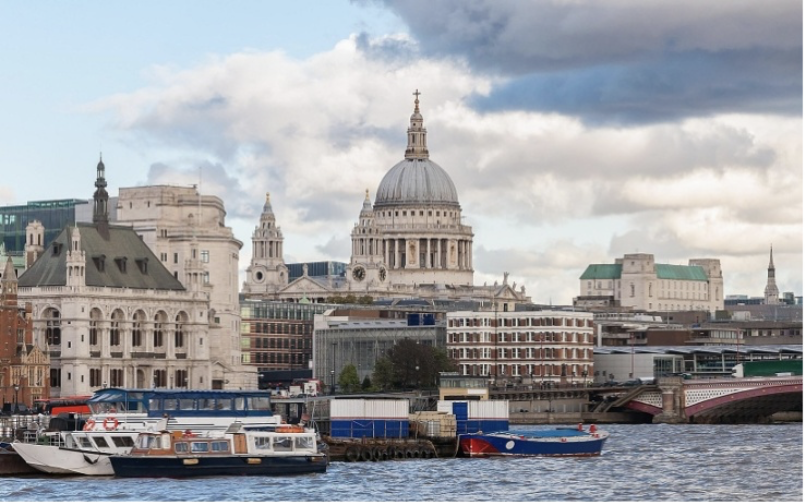
\includegraphics[width=1\linewidth]{images-task/real.png}
                \label{ris:graph}
            \end{minipage}
            \hfill
            \begin{minipage}[!h]{0.45\linewidth}
                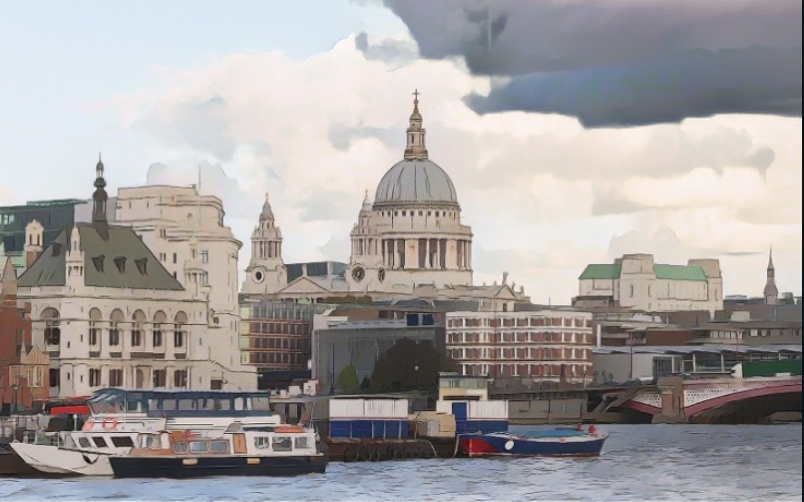
\includegraphics[width=1\linewidth]{images-task/processed.png}
                \label{ris:pbtxt}
            \end{minipage}
        \end{center}
        \caption{Пример использования модели whitebox\_cartoon\_gan для стилизации фото}
    \end{figure}
    
    Данные модели принимают тензор изображения в формате BGR со значениями в диапазоне $[-1.0; 1.0]$. Для реализации под macOS будет использована модель с входными данными $360 \times 640$. На платформах Linux и iOS будет задействована модель с входными данными $640 \times 360$ из-за особенности расположения дисплея на iOS.

    Итак, сформулируем задачу улучшения качества видеопотока с помощью нейронных сетей на графических процессорах, которая будет изучаться в данной работе. Необходимо разработать конвейеры для инференса выбранных моделей под платформы macOS, Linux и iOS. На вход будет предоставлен кадр с камеры устройства, на выходе - получен стилизированный кадр. Для тестирования работы конвейеров будут реализованы приложения на языках С++ и Swift под соответствующие платформы.

    \chapter{Обзор фреймворка MediaPipe. Основные элементы конвейера}
        \section{Знакомство с MediaPipe}
        MediaPipe — один из самых обширных фреймворков для запуска конвейеров (предобработка данных, запуск (inference) модели, постобработка результатов модели) машинного обучения, позволяющий упростить написание кроссплатформенного кода для запуска предобученных моделей. Эта структура может использоваться для различных приложений для обработки изображений и мультимедиа (особенно в виртуальной реальности), таких как обнаружение объектов, распознавание лиц, отслеживание рук, отслеживание нескольких рук и сегментация волос. MediaPipe поддерживает различные аппаратные и операционные платформы, такие как Android, iOS и Linux, предлагая API на C++, Java, Objective-c и т.д.

        В контексте поставленной задачи будет использован фреймворк MediaPipe на языке программирования C++ и Swift для платформ macOS, Linux и iOS.
        
        \section{Основные элементы конвейера}
        \subsection{Пакет (Packet)}
        Пакет (англ. Packet) — единица данных, перемещаемая по потокам и обрабатываемая калькулятором. Каждый пакет несёт в себе данные определённого типа — это может быть строка, целое число, массив чисел с плавающей запятой или пользовательский тип, описанный и сериализуемый в protobuf. Каждый пакет содержит в себе timestamp — отметку времени, ассоциированную с пакетом. Она напрямую не связана с реальным временем, так как нужна для того, чтобы отличать, какой пакет был раньше, какой позже. 
        
        \subsection{Узлы (Nodes or calculator)}
        Узлы (англ. Nodes) создают и/или обрабатывают Packet, и именно на них приходится основная часть работы графа. По историческим причинам их также называют calculator. У каждого калькулятора должен быть как минимум один входящий и как минимум один исходящий поток. Калькулятор представляет из себя C++ класс, реализующий интерфейс CalculatorBase:
        \begin{itemize}
          \item[-] \begin{verbatim}static ::mediapipe::Status GetContract(CalculatorContract*);\end{verbatim} статический метод, в котором калькулятор описывает форматы данных, которые ждет на вход и готов отдать на выход;
          
          \item[-] \begin{verbatim}::mediapipe::Status Open(CalculatorContext*);\end{verbatim} инициализация калькулятора при создании графа. Здесь, например, может быть загрузка данных, требуемых для работы;
          
          \item[-] \begin{verbatim}::mediapipe::Status Process(CalculatorContext*);\end{verbatim} обработка поступившего пакета;
          
          \item[-] \begin{verbatim}::mediapipe::Status Close(CalculatorContext*);\end{verbatim} 
           закрытие вершины.
        \end{itemize}
        
        \subsection{Поток (Streams)}
        Ребра графа (англ. Streams) задают связи между калькуляторами. С помощью потоков по графу перемещаются пакеты с данными. Поток может быть внутренним, входным (input) и исходящим (output). Внутренний поток соединяет два калькулятора, по входному потоку из внешнего кода в граф попадают данные, а с помощью исходящего потока граф отправляет данные наружу, в вызывающий код.

        \subsection{Граф (Graph)}
        Обработка данных в MediaPipe происходит внутри графа (англ. Graph), который определяет пути потока пакетов между узлами. Граф может иметь любое количество входов и выходов, а поток данных может разветвляться и сливаться. Как правило, данные идут вперед, но возможны и обратные циклы.
        \begin{figure}[h]
            \begin{center}
                \begin{minipage}[h]{0.3\linewidth}
                    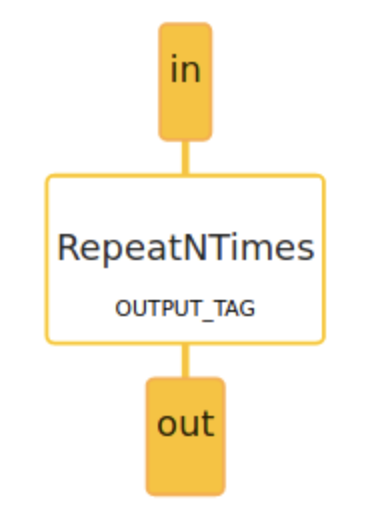
\includegraphics[width=0.5\linewidth]{images-mediapipe/graph.png}
                    \caption{Простейший граф (визуализация)}
                    \label{ris:graph}
                \end{minipage}
                \hfill
                \begin{minipage}[h]{0.5\linewidth}
                    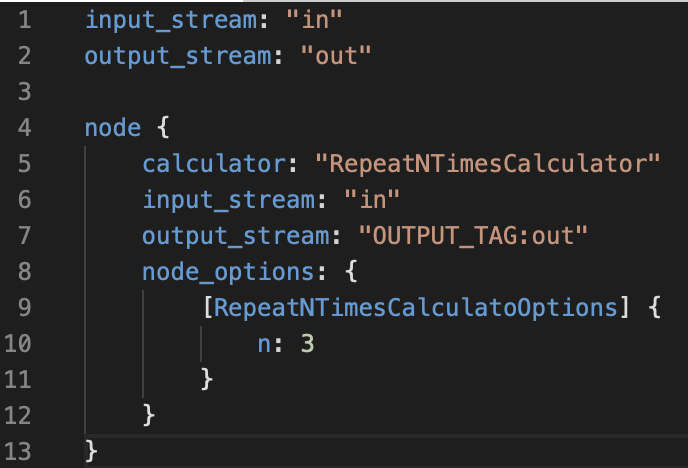
\includegraphics[width=0.7\linewidth]{images-mediapipe/pbtxt.png}
                    \caption{Простейший граф (pbtxt)}
                    \label{ris:pbtxt}
                \end{minipage}
            \end{center}
        \end{figure}

        \subsection{Конвейер (Pipeline)}
        Конвейер в MediaPipe задается в форме графа. Графы описываются в формате protobuf text file (pbtxt). MediaPipe позволяет из калькуляторов составлять необходимый конвейер для запуска модели, а затем просто встраивать его в приложения на разных платформах. Сейчас разработчики заявляют о поддержке нескольких дистрибутивов Linux, WSL, MacOS, Android, iOS. В MediaPipe есть встроенные калькуляторы для запуска TensorFlow и TFLite моделей.
        \begin{figure}[h]
            \center{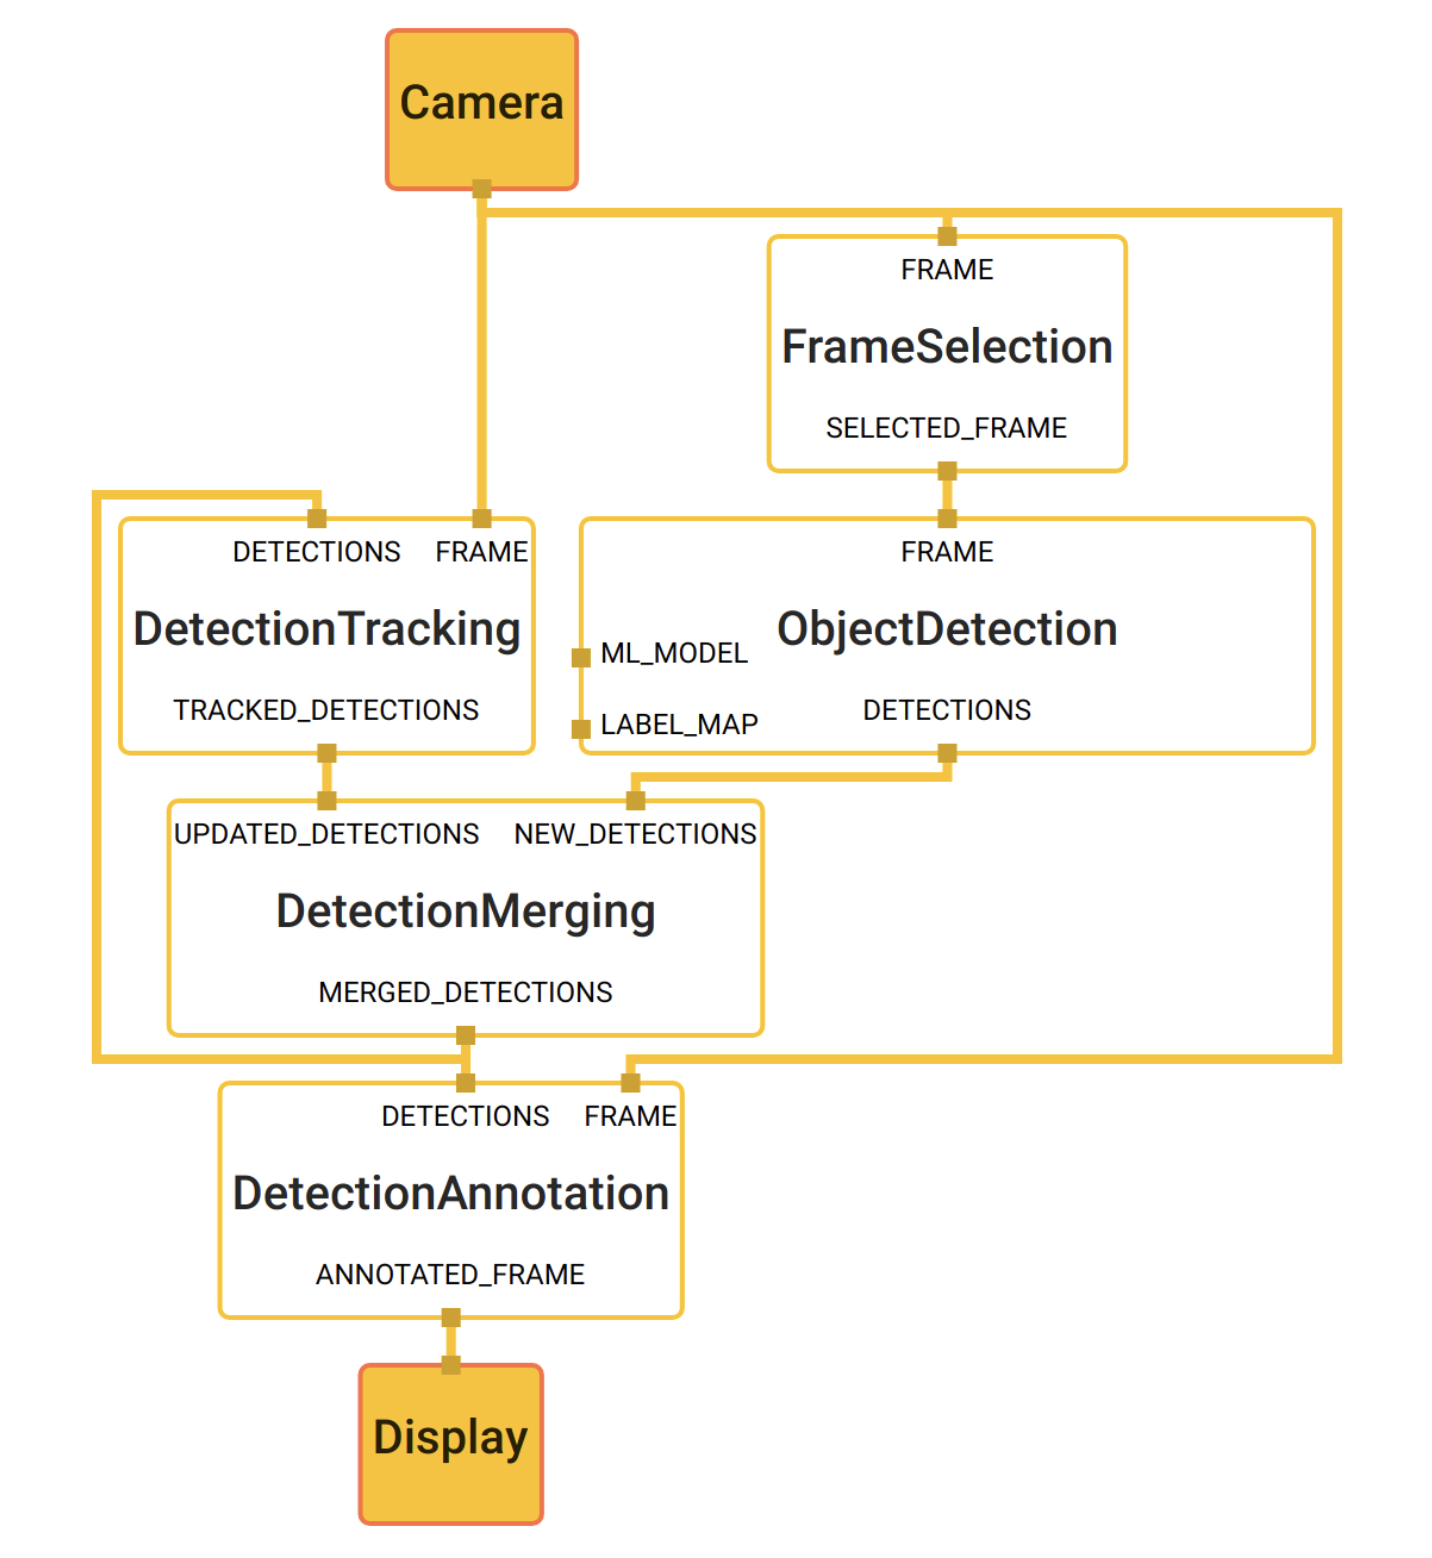
\includegraphics[width=1\linewidth]{images-task/pipiline.png}}
            \caption{Пример конвейера}
            \label{ris:subgraph}
        \end{figure}

    \chapter{Разработка конвейера улучшения видеопотока}
        \section{Разработка архитектуры конвейера}
        Для запуска модели необходимо создать конвейер, который в случае с фреймворком MediaPipe представляет собой граф из некоторого количества калькуляторов. В этом пункте определим архитектуру общего конвейера, а в следующих внесем коррективы для определённых платформ и сетей.

        На вход в конвейер будет поступать текущее изображение видеопотока. На выходе конвейер будет возвращать текущий кадр с примененными улучшениями. В зависимости от платформы тип входного изображения будет изменяться. Так на Linux и iOS в конвейер будет поступать кадр типа mediapipe::GpuBuffer, на macOS же будет поступать кадр типа mediapipe::ImageFrame.
        \lstinputlisting[caption={Инициализация входных пакетов в графе конвейера}]{codePipeline/input.proto}

        Для предотвращения скопления узлов в очередь на получение изображений и данных (это приводило бы к увеличению задержек и расходу памяти) используется калькулятор FlowLimiterCalculator. Кроме того, данный калькулятор устраняет ненужные вычисления, например, вывод, произведенный узлом, может быть передан далее по потоку, если последующие узлы все еще заняты обработкой предыдущих входных данных. Для управления потоком калькулятор пропускает первое входящее изображение без изменений и ждет, пока нижележащие узлы графа (калькуляторы или подграфы) не закончат свои вычисления, прежде чем пропустить еще одно изображение.

        На вход данный калькулятор принимает текущий кадр видеопотока и поток FINISHED от указанного калькулятора конвейера. Так как последний калькулятор конвейера будет лишь переводить из одного формата в другой и это не будет занимать много времени, необходимо ждать выполнения \hyperlink{TensorToImage}{калькулятора преобразования тензора в изображение}. В input\_stream\_info ставится параметр, который указывает, в каком состоянии должен быть поток FINISHED, для того чтобы калькулятор пропустил следующее изображение. Если поток FINISHED будет не пустым, калькулятор передаст следующее изображение, иначе они будут отбрасываться.
        \lstinputlisting[caption={Вызов калькулятора FlowLimiterCalculator в графе конвейера}]{codePipeline/flow.proto}

        После получения отфильтрованного кадра в пакет throttled\_input\_video нужно провести необходимую обработку для получения подходящего на вход модели тензора. Для этого используется калькулятор ImageToTensorCalculator. Данный калькулятор является универсальным и даёт возможность получить входной тензор для кадра любого типа (ImageFrame и GpuBuffer). Это возможно, так как этот калькулятор реализован на Metal (для iOS), OpenGL (для Linux), OpenCV (для macOS).

        На вход калькулятор ImageToTensorCalculator принимает текущий кадр из FlowLimiterCalculator. Возвращает готовый для инференса тензор. Во время превращения изображение подготавливается в подходящий для модели формат. Для этого указываются дополнительные параметры:
        \begin{itemize}
          \item[-] \textbf{output\_tensor\_width} ширина ожидаемого на вход модели изображения;
          \item[-] \textbf{output\_tensor\_heigth} высота ожидаемого на вход модели изображения;
          \item[-] \textbf{keep\_aspect\_ratio} устанавливает нужно ли при переходе ко входным размерам модели сохранять соотношение сторон как у исходного изображения;
          \item[-] \textbf{output\_tensor\_float\_range} указывает минимальное и максимальное ожидаемые значения типа float;
          \item[-] \textbf{gpu\_origin} указывает, как расположено изображение. Для OpenGL входное изображение начинается снизу и его нужно перевернуть по вертикали, так как тензоры должны начинаться сверху;
          \item[-] \textbf{border\_mode} указывает метод пиксельной экстраполяции. При преобразовании изображения в тензор может произойти, что тензору потребуется считать пиксели за пределами границ изображения. Этот параметр указывает, как такие пиксели будут вычисляться.
        \end{itemize}
        \lstinputlisting[caption={Вызов калькулятора ImageToTensorCalculator в графе конвейера}]{codePipeline/ImageToTensor.proto}

        Далее полученный тензор отправляется на инференс модели. Для этого используется калькулятор InferenceCalculator. На вход данный калькулятор принимает тензор входного изображения в подходящем размере. Возвращает данный калькулятор тензор обработанного изображения. Дополнительно указывается путь до модели, которая будет использована в данном графе, и делегат, который будет отвечать за запуск модели. Этот калькулятор можно считать универсальным и не зависящим от платформы, так как он поддерживает реализацию таких делегатов, как XNNPack (для любого CPU, но в этом случае для macOS) и GPU (Metal для iOS и OpenGL для Linux).
        \lstinputlisting[caption={Вызов калькулятора InferenceCalculator в графе конвейера}]{codePipeline/inference.proto}

        На следующем шаге тензор, полученный от InferenceCalculator, восстанавливается в выходное изображение. Для этого используется калькулятор \hypertarget{TensorToImage}{TensorToImageCalculator}. На вход он принимает тензор для восстановления. Возвращает изображение формата mediapipe::Image. Для корректного восстановления изображения из тензора необходимо указать дополнительные параметры:
        \begin{itemize}
          \item[-] \textbf{gpu\_origin} указывает, как расположено изображение. Для OpenGL входное изображение начинается снизу и его нужно перевернуть по вертикали, так как тензоры должны начинаться сверху;
          \item[-] \textbf{input\_tensor\_float\_range:min} минимальное ожидаемое значение типа float;
          \item[-] \textbf{input\_tensor\_float\_range:max} максимальное ожидаемое значение типа float;
          \item[-] \textbf{tensor\_position} указывает какой входной тензор нарезать, если в модели несколько выходных тензоров.
        \end{itemize}
        Данный калькулятор также является универсальным, так как реализован на Metal (для iOS), OpenGL (для Linux) и OpenCV (для macOS).
        \lstinputlisting[caption={Вызов калькулятора TensorToImageCalculator в графе конвейера}]{codePipeline/TensorToImage.proto}

        Для получения итогового изображения осталось перевести, полученное в калькуляторе TensorToImageCalculator, из формата mediapipe::Image в mediapipe::ImageFrame для CPU на macOS и в mediapipe::GpuBuffer для GPU на iOS и Linux. Для этого используется калькулятор FromImageCalculator.
        \lstinputlisting[caption={Вызов калькулятора FromImageCalculator в графе конвейера}]{codePipeline/FromImage.proto}
        
        На данном калькуляторе описание общей архитектуры конвейера заканчивается. Для лучшего понимания полноценной архитектуры прилагается визуализированный граф конвейера (рис \ref{ris:graph})
        \begin{figure}[!h]
            \center{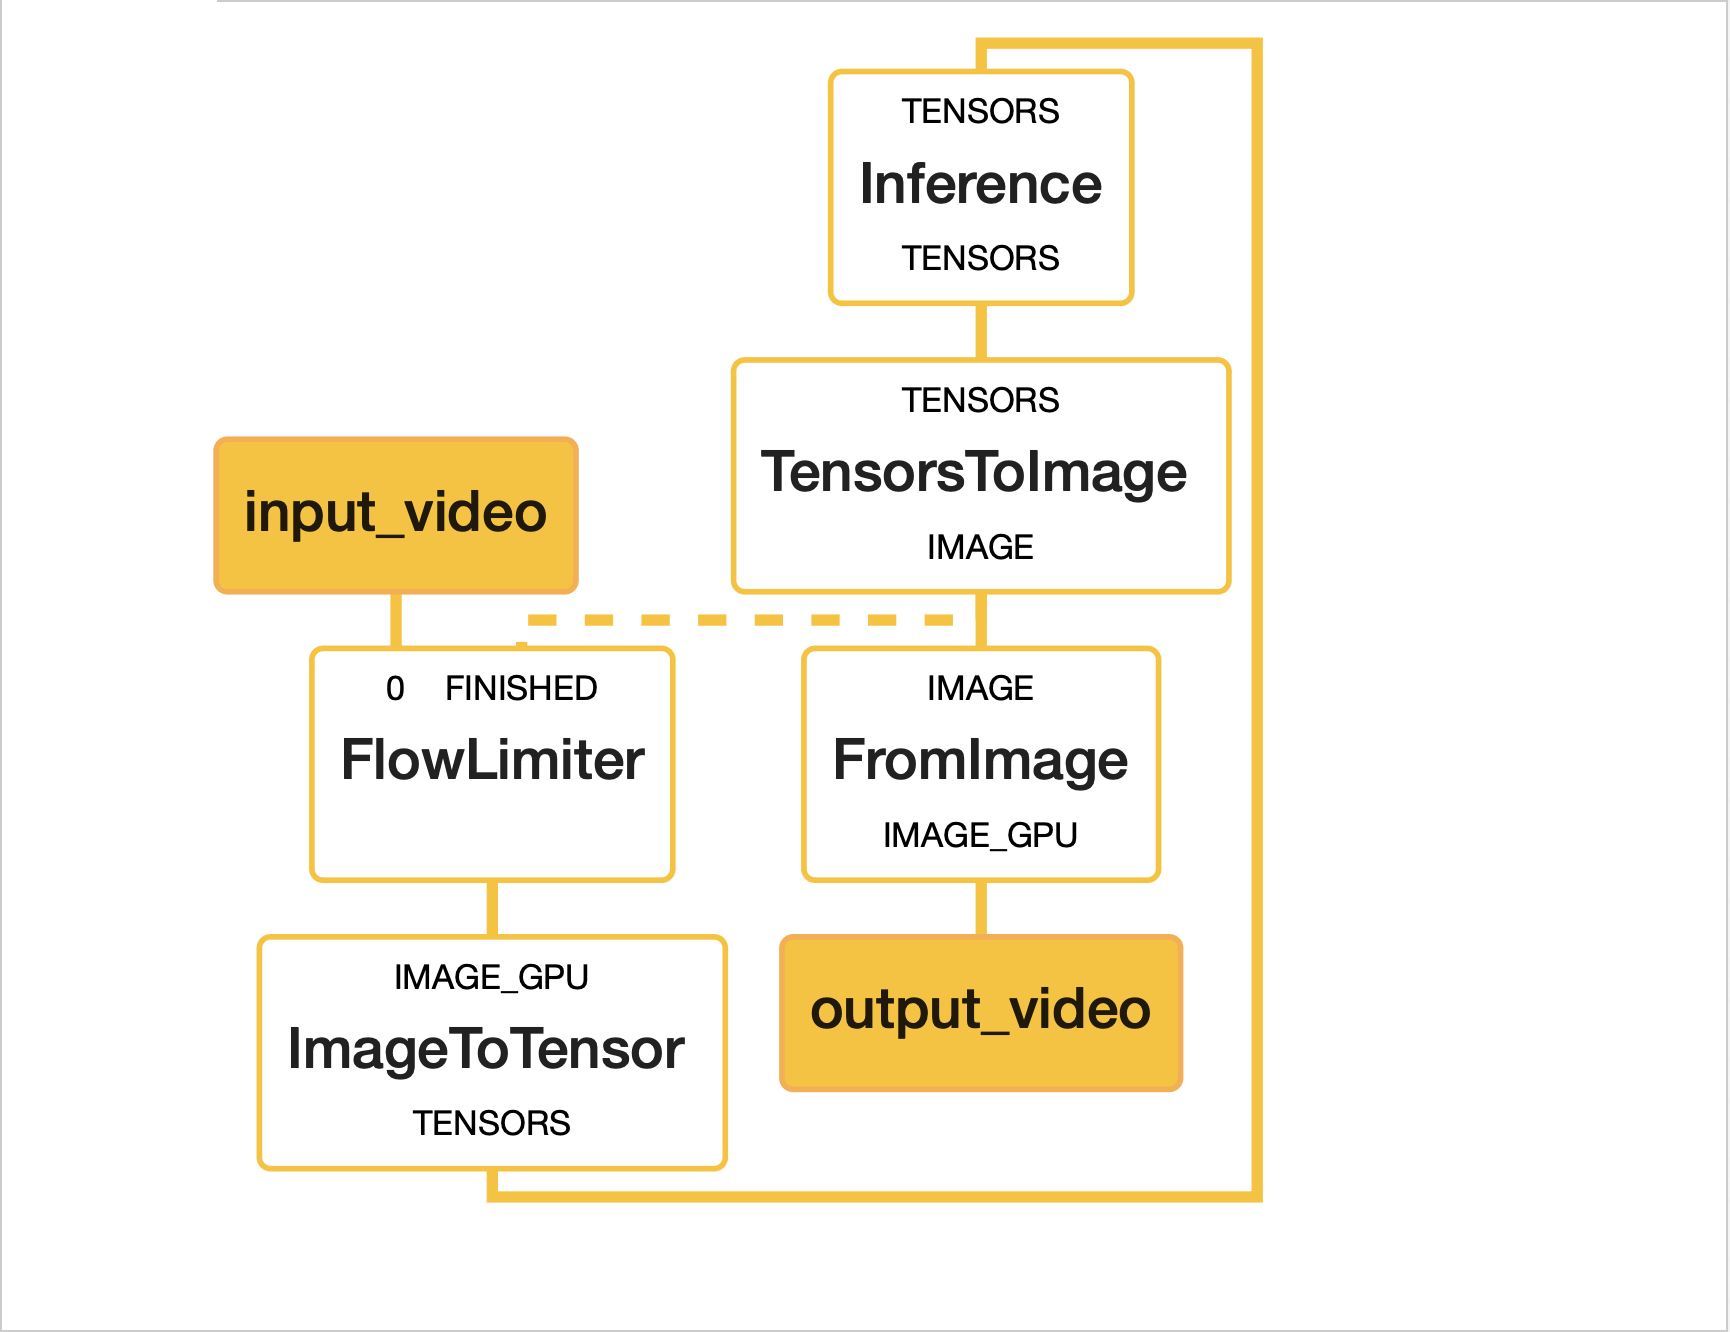
\includegraphics[width=1\linewidth]{images-pipeline/graph.png}}
            \caption{Граф конвейера улучшения качества видеопотока}
            \label{ris:graph}
        \end{figure}
        Далее рассмотрим конкретные графы для macOS, iOS и Linux.
        
        \section{Конвейер для улучшения качества видеопотока на macOS}
        Так как для стилизации была выбрана модель whitebox\_cartoon\_gan и данный инференс будет проходить на CPU и платформе macOS, граф будет реализован под landscape разрешение, а именно $360 \times 540$. Таким образом, конвейер будет иметь вид:
        \lstinputlisting[caption={Граф для стилизации на macOS}]{codePipeline/CartoonMacOS.proto}

        \section{Конвейер для улучшения качества видеопотока на iOS и Linux}
        Так как для стилизации была выбрана модель whitebox\_cartoon\_gan и данный инференс будет проходить на GPU, на платформах Linux и iOS (граф для них абсолютно одинаковый), граф будет реализован под portrait разрешение, а именно $540 \times 360$. Таким образом, конвейер будет иметь вид:
        \lstinputlisting[caption={Граф для стилизации на Linux и iOS}]{codePipeline/CartoonGpu.proto}
    
    \chapter{Реализация приложений для запуска графов}
        \section{Запуск графа на macOS и Linux}
        Для запуска графов на macOS и Linux необходимо реализовать простейшее приложение, которое будет принимать кадр с камеры и выводить его на экран. Разница между реализациями на macOS и Linux будет заключаться лишь в том, что на первой платформе в граф будет передано изображение из CpuBuffer'а, а именно mediapipe::ImageFrame, а на второй из mediapipe::GpuBuffer'а.

        В самом начале необходимо загрузить и инициализировать конвейер. Он будет передаваться посредством указания пути в параметрах при запуске тестового приложения. Далее подгружается камера. Эта часть общая у обеих платформ. Код приведен ниже.
        \lstinputlisting[language=c++, caption={Инициализация графа и камеры}]{codeApplication/InitGraph.cpp}

        Далее на Linux необходимо инициализировать GPU. Для этого создаются GpuResources и GpuHelper. Код приведен ниже.
        \lstinputlisting[language=c++, caption={Инициализация GPU на Linux}]{codeApplication/InitGpu.cpp}

        Затем идет общая часть для двух платформ: запускается граф. Для этого создается \hypertarget{poller}{Poller}. С его помощью данные из выходного потока графа будут возвращены в приложение. В данном случае он следит за потоком с названием "output\_video". Затем происходит непосредственный запуск графа. Так как в графе нет input\_side\_packets, то в функцию StartRun не передается никаких параметров.
        \lstinputlisting[language=c++, caption={Запуск графа}]{codeApplication/StartGraph.cpp}

        Далее начинается цикл обработки кадров с камеры. Так как модель whitebox\_cartoon\_gan \hyperlink{[2]}{[2]} принимает на вход изображение в формате BGR, и кадр с камеры захватывается с помощью OpenCV, переводить кадр из RGB в BGR не нужно. Из-за того, что выполнение цикла может начаться до окончательной инициализации камеры, пустые кадры необходимо пропустить. Далее кадр поворачивается вертикально на 180 градусов (особенность OpenCV) и передается в функцию \hyperlink{send}{SendFrameToGraph}. Реализация этой функции будет отличаться на macOS и Linux. Рассмотрим её позже.
        
        После выполнения данной функции, возвращается кадр из графа. Для этого используется \hyperlink{get}{GetOutput}. Эта функция также будет отличаться на каждой из платформ.

        В конце цикла выводится на экран полученный из графа кадр и стоит проверка на закрытие приложения. Код всего цикла приведен ниже.
        \lstinputlisting[language=c++, caption={Цикл обработки кадров с камеры}]{codeApplication/While.cpp}

        Реализация функции \hypertarget{send}{SendFrameToGraph} на macOS довольно проста. Кадр, захваченный с камеры, переводится из формата cv::Mat в формат mediapipe::ImageFrame. Затем рассчитывается текущая метка времени (FrameTimestampUs) и вместе с конвертированным кадром передаются в граф.
        \lstinputlisting[language=c++, caption={Реализация функции SendFrameToGraph на macOS}]{codeApplication/SendCpu.cpp}

        Реализация \hypertarget{send}{SendFrameToGraph} на Linux немного отличается. Сперва кадр переводится из cv::Mat в формат mediapipe::ImageFrame. Затем задействованы вспомогательные функции для перевода кадра из формата mediapipe::ImageFrame в mediapipe::GpuBuffer. Далее, с рассчитанной меткой времени, кадр посылается в граф.
        \lstinputlisting[language=c++, caption={Реализация функции SendFrameToGraph на Linux}]{codeApplication/SendGpu.cpp}

        Функция \hypertarget{get}{GetOutput} на macOS забирает пакет из \hyperlink{poller}{Poller}, получает кадр в формате mediapipe::ImageFrame. Переводит из формата mediapipe::ImageFrame в cv::Mat.
        \lstinputlisting[language=c++, caption={Реализация функции GetOutput на macOS}]{codeApplication/GetCpu.cpp}

        Функция \hypertarget{get}{GetOutput} на Linux забирает пакет из \hyperlink{poller}{Poller}, получает кадр в формате mediapipe::GpuBuffer и считывает из framebuffer'а OpenGl контекста в OutputFrame (формат mediapipe::ImageFrame). Затем переводит из формата mediapipe::ImageFrame в cv::Mat. Если выходное изображение имеет 4 канала, переводим из RGBA в RGB.
        \lstinputlisting[language=c++, caption={Реализация функции GetOutput на Linux}]{codeApplication/GetGpu.cpp}
        
        После выполнения цикла обработки кадров вызываются функции для закрытия графа, сеанса и камеры.
        \lstinputlisting[language=c++, caption={Закрытие графа и сеанса}]{codeApplication/End.cpp}

        Описание кода закончено. Осталось его собрать и протестировать. Ниже приведены примеры работы собранного приложения под MacOS и Linux:
        \begin{figure}[h]
            \begin{center}
                \begin{minipage}[h]{0.4\linewidth}
                    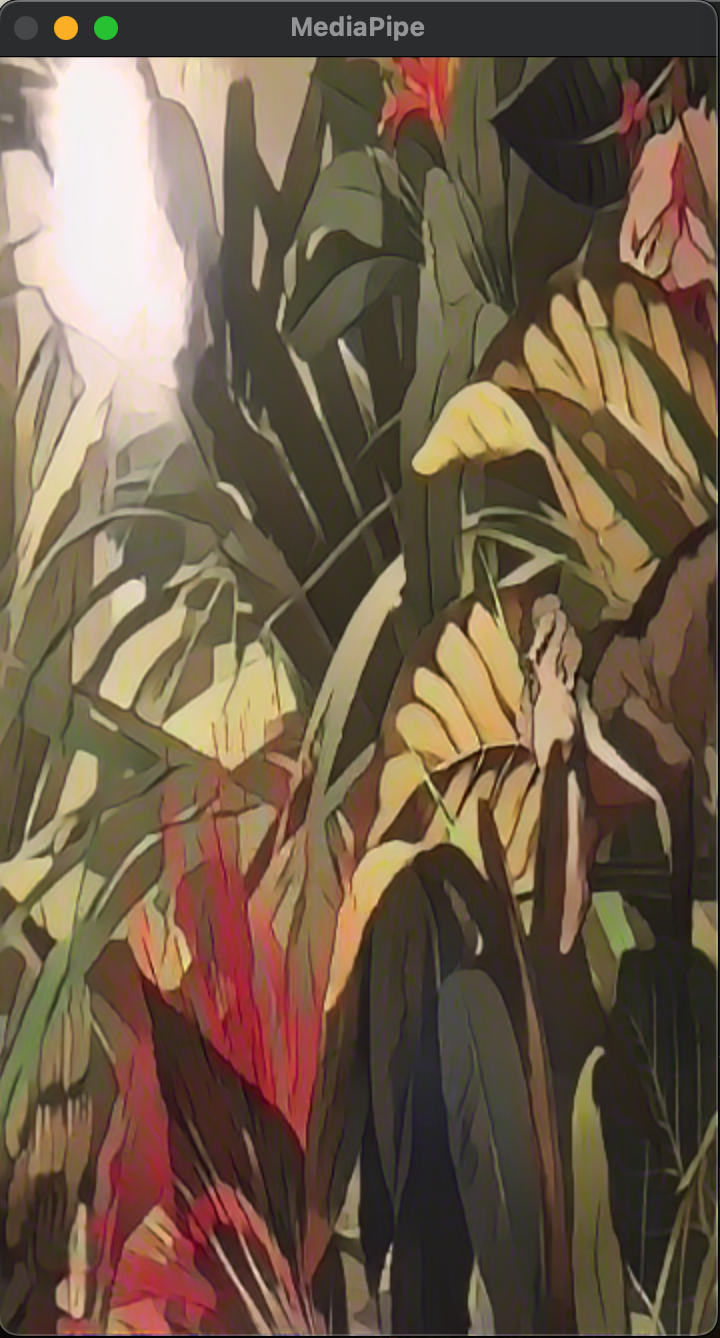
\includegraphics[width=1\linewidth]{images-code/Linux.png}
                    \caption{Работа приложения на Linux}
                    \label{ris:graph}
                \end{minipage}
                \hfill
                \begin{minipage}[h]{0.5\linewidth}
                    
\includegraphics[width=1\linewidth]{images-code/macOS.png}
                    \caption{Работа приложения на macOS}
                    \label{ris:pbtxt}
                \end{minipage}
            \end{center}
        \end{figure}

        \section{Запуск графа на iOS}
        Чтобы запустить граф на iOS, разработаем приложение. Для этого необходимо собрать библиотеку на основе MediaPipe. С этой целью был создан следующий файл сборки:
        \lstinputlisting[caption={Файл сборки библиотеки под iOS}]{codeApplication/BUILD}

        \hypertarget{delegate}{Так} как на iOS используется Metal, необходимо сделать "прослойку" для корректной работы графа из фреймворка MediaPipe. Для этого был реализован интерфейс VideoProcessor для связи MediaPipe и iOS приложения. В данном файле присутствует делегат для обработки кадра, интерфейс, инициализирующий, запускающий граф, и функция обработки кадра. Также данный интерфейс хранит делегат и метку времени.
        \lstinputlisting[language=c++, caption={Интерфейс для связи MediaPipe и iOS приложения}]{codeApplication/Obj.h}

        Далее были реализованы данные функции:
        \begin{enumerate}
            \item Функция для очистки всех параметров. Закрывает граф, входной и выходной потоки, и удостоверяется, что все ресурсы очищены. Предотвращает утечки памяти.\lstinputlisting[language=c++, caption={Функция для очистки всех параметров}]{codeApplication/CleanUp.mm}
            \item Функция инициализации графа из ресурсов приложения.\lstinputlisting[language=c++, caption={Функция загрузки графа из ресурсов приложения}]{codeApplication/Init.mm}
            \item Вспомогательная функция загрузки графа из ресурсов приложения. После загрузки его инициализируют и запускают. Так как в графе нет input\_side\_packet, указываются только входной и выходной поток.\lstinputlisting[language=c++, caption={Вспомогательная функция загрузки графа из ресурсов приложения}]{codeApplication/LoadGraph.mm}
            \item Функция запуска графа. Если при запуске графа на стороне MediaPipe возникает ошибка, она выводится в приложении. Иначе выводится лог о старте графа.\lstinputlisting[language=c++, caption={Функция запуска графа}]{codeApplication/Start.mm}
            \item Функция делегата. Оповещает приложение о получении выходного изображения из графа и перенаправляет изображение в приложение.\lstinputlisting[language=c++, caption={Функция делегата}]{codeApplication/Delegate.mm}
            \item Функция обработки кадра. Отправляет кадр во входной поток графа MediaPipe. При возникновении ошибок на любом из этапов, выводит ее в лог и заканчивает работу конвейера.\lstinputlisting[language=c++, caption={Функция обработки кадра}]{codeApplication/Process.mm}
        \end{enumerate}

        После сборки библиотеки, необходимо применить скрипт patch\_framevork.sh для получения нужного файла. Для работы с библиотекой, собранной при помощи MediaPipe, надо добавить файл module.modulemap и файлы заголовков. Это необходимо для загрузки всех зависимостей в проект XCode. Ниже представлен код скрипта:
        \lstinputlisting[language=c++, caption={Скрипт окончательной сборки библиотеки}]{codeApplication/Patch.sh}

        Далее был создан новый проект в XCode под платформу iOS. В полученном проекте класс AppDelegate был заменен на предоставляемый в MediaPipe. В обновленном классе добавлены функции, которые описывают стандартное поведение приложения, переведенного в фоновый режим. Кроме того, в главном окне приложения устанавливается основной контроллер: StylisingViewController.
        \lstinputlisting[language=swift, caption={Код обновленного класса AppDelegate}]{codeApplication/App.swift}

        Для работы с камерой устройства был реализован класс Camera. В данном классе происходит инициализация камеры. Также реализованы функции для старта сессии работы с камерой (start), для завершения работы камеры (stop). Помимо этого была создана функция для передачи текущего кадра \hyperlink{delegate}{делегату} графа MediaPipe и функция смены передней/задней камеры. Так как на вход граф ожидает изображение в формате BGR, запрашиваем у камеры именно такой формат.
        \lstinputlisting[language=swift, caption={Класс Camera для работы с камерой}]{codeApplication/Cameras.swift}

        Основная логика приложения заключена в классе контроллера StylisingViewController. У данного класса присутствуют атрибуты:
        \begin{enumerate}
            \item \textbf{camera} — хранит объект камеры и отвечает за передачу кадра из камеры устройства в граф;
            \item \textbf{displayLayer} — объект типа AVSampleBufferDisplayLayer, который может транслировать кадр из камеры на экран, как только они поступают. Работает напрямую с буфером камеры, что повышает скорость;
            \item \textbf{videoProcessor} — объект класса VideoProcessor, который отвечает за работу с графом MediaPipe. Для этого был создан класс \hyperlink{delegate}{VideoProcessor};
            \item \textbf{cameraView} — элемент UI для размещения кадра, полученного напрямую из displayLayer;
            \item \textbf{imgView} — элемент UI для размещения обработанного VideoProcessor кадра;
            \item \textbf{switchCameraButton} — кнопка для смены камеры. Доступно два варианта: фронтальная (по умолчанию) и задняя.
        \end{enumerate}
        \lstinputlisting[language=swift, caption={Атрибуты классы StylisingViewController}]{codeApplication/Attributes.swift}
        
        Далее реализуются основные функции. Первая из них viewDidLoad. Данная функция отвечает за инициализацию и активацию контроллеров и элементов UI. Таким образом настраивается imgView, который занимает весь экран приложения, и кнопка для смены камеры. Также запускаются камера и граф обработки кадра на стороне MediaPipe.
        \lstinputlisting[language=swift, caption={Функция viewDidLoad}]{codeApplication/DidLoad.swift}

        Далее реализованы функции viewDidLayoutSubviews и didTapSwitchCamera. Первая удостоверяется, что displayLayer установлен в корректный размер и совпадает с cameraView. didTapSwitchCamera отвечает за нажатие на кнопку смены камеры и, при нажатии, переводит с одной камеры на другую.
        \lstinputlisting[language=swift, caption={Функции viewDidLayoutSubviews и didTapSwitchCamera}]{codeApplication/DidLayout.swift}

        Функция captureOutput отвечает за передачу кадров с камеры на конвейер MediaPipe. В данной функции конкретно устанавливается режим работы в portrait формате.
        \lstinputlisting[language=swift, caption={Функция captureOutput}]{codeApplication/DidCapture.swift}
        
        Функция didProcessFrame забирает кадры из выходного потока графа MediaPipe и выводит их на экран приложения.
        \lstinputlisting[language=swift, caption={Функция didProcessFrame}]{codeApplication/DidProcess.swift}

        Это был последний класс, который был необходим для работы приложения. Осталось его собрать и протестировать. Ниже приведена работа собранного приложения под iOS:
        \begin{figure}[h]
            \center{\includegraphics[width=0.3\linewidth]{images-code/iOS.png}}
            \caption{Работа приложения под iOS}
            \label{ris:subgraph}
        \end{figure}

    \chapter*{Заключение}
    \addcontentsline{toc}{chapter}{Заключение}
    В ходе работы:
    \begin{enumerate}
        \item Была рассмотрена задача улучшения видеопотока с помощью фреймворка MediaPipe, а также ее применение на прикладном уровне;
        \item Сделан краткий обзор фреймворка MediaPipe;
        \item Выполнен обзор основных элементов конвейера фреймворка MediaPipe;
        \item Разработана общая архитектура конвейера;
        \item Реализованы конвейеры для платформ macOS, Linux и iOS;
        \item Разработаны приложения для тестирования конвейеров на macOS, Linux и iOS на языках программирования C++ и Swift;
        \item Успешно протестированы результаты работы.
    \end{enumerate}

    \chapter*{Список использованных источников}
    \addcontentsline{toc}{chapter}{Список использованных источников}
    \begin{enumerate}
        \item Lugaresi.C., Tang.J., Nash.H., McClanahan.C., Uboweja.E., Hays.M., Zhang.F., Chang.C.-L., Yong.M.G., Lee.J., Chang.W.-T., Hua.W., Georg.M., Grundmann.M. (2019). MediaPipe: A Framework for Perceiving and Processing Reality [Электронный ресурс]: CVPR CV4ARVR Workshop 2019/Google Research. – Mountain View, CA: Google Research, 2019. – Режим доступа: \href{https://static1.squarespace.com/static/5c3f69e1cc8fedbc039ea739/t/5e130ff310a69061a71cbd7c/1578307584840/NewTitle_May1_MediaPipe_CVPR_CV4ARVR_Workshop_2019.pdf}{https://static1.squarespace.com/static/5c3f69e1cc8fedbc039ea739/t/5e130f\\f310a69061a71cbd7c/1578307584840/NewTitle\_May1\_MediaPipe\_CVPR\\\_CV4ARVR\_Workshop\_2019.pdf}. – Дата доступа: 18.12.2024.
        \item \hypertarget{[2]}{}Wang.X., Yu.J. (2020). Learning to Cartoonize Using White-box Cartoon Representations [Электронный ресурс]: CVPR 2020/ByteDance, The University of Tokyo, Style2Paints Research. – Mountain View, CA: ByteDance, 2020. – Режим доступа: \href{https://openaccess.thecvf.com/content_CVPR_2020/papers/Wang_Learning_to_Cartoonize_Using_White-Box_Cartoon_Representations_CVPR_2020_paper.pdf}{https://openaccess.thecvf.com/content\_CVPR\_2020/papers/Wang\_Lear\\ning\_to\_Cartoonize\_Using\_White-Box\_Cartoon\_Representations\_CVP\\R\_2020\_paper.pdf}. – Дата доступа: 18.12.2024.
        \item Sharma.S., Kama.S., Bernauer.J., Moroney.L. (2018). Speed up TensorFlow Inference on GPUs with TensorRT [Электронный ресурс]: The TensorFlow Blog / NVidia. – Город издания: NVidia, 2018. – Режим доступа: \href{https://blog.tensorflow.org/2018/04/speed-up-tensorflow-inference-on-gpus-tensorRT.html}{https://blog.tensorflow.org/2018/04/speed-up-tensorflow-inference-on-gpus-tensorRT.html}. – Дата доступа: 18.12.2024.
        \item Google. (2023). MediaPipe Framework [Electronic resource]: Google for Developers. Режим доступа: \href{https://developers.google.com/mediapipe/framework}{https://developers.google.com/mediapipe/framework}. Дата доступа: 18.12.2024
        \item TensorFlow. (2023). Segmentation [Electronic resource]: TensorFlow Lite. Режим доступа: \href{https://www.tensorflow.org/lite/examples/segmentation/overview}{https://www.tensorflow.org/lite/examples/segmentation/overview}. Дата доступа: 18.12.2024
        \item bazel.build. Bazel [Electronic resource]. Режим доступа: \href{https://bazel.build}{https://bazel.build}. Дата доступа: 18.12.2024
    \end{enumerate}
    
\end{document}
